\section{stat\_\-stat\_\-t Struct Reference}
\label{structstat__stat__t}\index{stat\_\-stat\_\-t@{stat\_\-stat\_\-t}}
{\tt \#include $<$stats.h$>$}

Collaboration diagram for stat\_\-stat\_\-t:\nopagebreak
\begin{figure}[H]
\begin{center}
\leavevmode
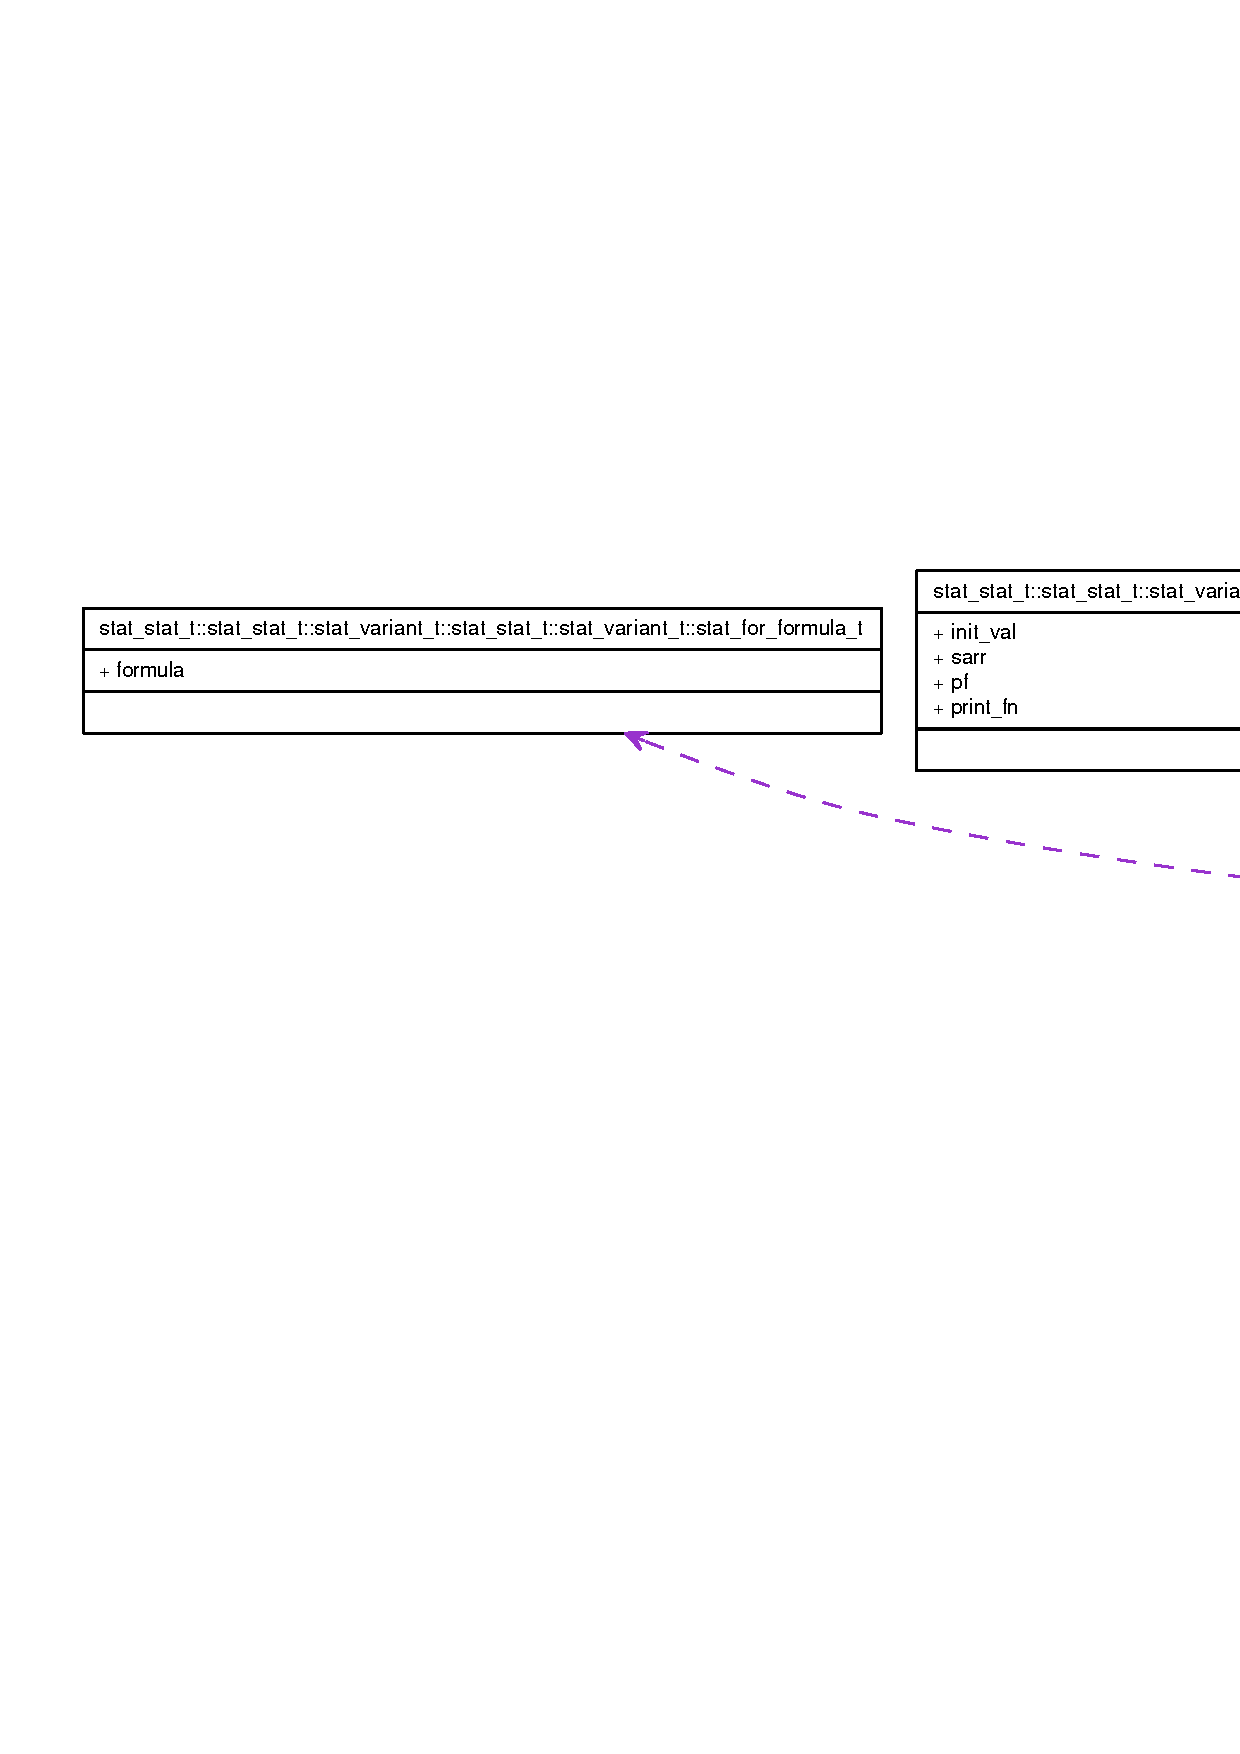
\includegraphics[width=400pt]{structstat__stat__t__coll__graph}
\end{center}
\end{figure}
\subsection*{Classes}
\begin{CompactItemize}
\item 
union {\bf stat\_\-variant\_\-t}
\end{CompactItemize}
\subsection*{Public Attributes}
\begin{CompactItemize}
\item 
struct {\bf stat\_\-stat\_\-t} $\ast$ {\bf next}
\item 
const char $\ast$ {\bf name}
\item 
const char $\ast$ {\bf desc}
\item 
const char $\ast$ {\bf format}
\item 
enum {\bf stat\_\-class\_\-t} {\bf sc}
\item 
int {\bf print\_\-me}
\item 
union {\bf stat\_\-stat\_\-t::stat\_\-variant\_\-t} {\bf variant}
\end{CompactItemize}


\subsection{Detailed Description}


Definition at line 122 of file zesto/stats.h.

\subsection{Member Data Documentation}
\index{stat\_\-stat\_\-t@{stat\_\-stat\_\-t}!desc@{desc}}
\index{desc@{desc}!stat_stat_t@{stat\_\-stat\_\-t}}
\subsubsection[{desc}]{\setlength{\rightskip}{0pt plus 5cm}const char$\ast$ {\bf stat\_\-stat\_\-t::desc}}\label{structstat__stat__t_bd10a35fb99e5a028095882d37ca2309}




Definition at line 125 of file zesto/stats.h.\index{stat\_\-stat\_\-t@{stat\_\-stat\_\-t}!format@{format}}
\index{format@{format}!stat_stat_t@{stat\_\-stat\_\-t}}
\subsubsection[{format}]{\setlength{\rightskip}{0pt plus 5cm}const char$\ast$ {\bf stat\_\-stat\_\-t::format}}\label{structstat__stat__t_cb226be68234f23178a842e1a4acf8cd}




Definition at line 126 of file zesto/stats.h.\index{stat\_\-stat\_\-t@{stat\_\-stat\_\-t}!name@{name}}
\index{name@{name}!stat_stat_t@{stat\_\-stat\_\-t}}
\subsubsection[{name}]{\setlength{\rightskip}{0pt plus 5cm}const char$\ast$ {\bf stat\_\-stat\_\-t::name}}\label{structstat__stat__t_68865d7221abe93b4b3c331e192f0d38}




Definition at line 124 of file zesto/stats.h.\index{stat\_\-stat\_\-t@{stat\_\-stat\_\-t}!next@{next}}
\index{next@{next}!stat_stat_t@{stat\_\-stat\_\-t}}
\subsubsection[{next}]{\setlength{\rightskip}{0pt plus 5cm}struct {\bf stat\_\-stat\_\-t}$\ast$ {\bf stat\_\-stat\_\-t::next}\hspace{0.3cm}{\tt  [read]}}\label{structstat__stat__t_96bb6646d86da1836eff66d9e4969cb7}




Definition at line 123 of file zesto/stats.h.\index{stat\_\-stat\_\-t@{stat\_\-stat\_\-t}!print\_\-me@{print\_\-me}}
\index{print\_\-me@{print\_\-me}!stat_stat_t@{stat\_\-stat\_\-t}}
\subsubsection[{print\_\-me}]{\setlength{\rightskip}{0pt plus 5cm}int {\bf stat\_\-stat\_\-t::print\_\-me}}\label{structstat__stat__t_9f0a547ad6eacd4d8192c026eb61753c}




Definition at line 128 of file zesto/stats.h.\index{stat\_\-stat\_\-t@{stat\_\-stat\_\-t}!sc@{sc}}
\index{sc@{sc}!stat_stat_t@{stat\_\-stat\_\-t}}
\subsubsection[{sc}]{\setlength{\rightskip}{0pt plus 5cm}enum {\bf stat\_\-class\_\-t} {\bf stat\_\-stat\_\-t::sc}}\label{structstat__stat__t_0bc6f92d0330183b00c273b917c83a21}




Definition at line 127 of file zesto/stats.h.\index{stat\_\-stat\_\-t@{stat\_\-stat\_\-t}!variant@{variant}}
\index{variant@{variant}!stat_stat_t@{stat\_\-stat\_\-t}}
\subsubsection[{variant}]{\setlength{\rightskip}{0pt plus 5cm}union {\bf stat\_\-stat\_\-t::stat\_\-variant\_\-t}  {\bf stat\_\-stat\_\-t::variant}}\label{structstat__stat__t_f97c4cea4ea2372a78b0ae1f94db25ac}




The documentation for this struct was generated from the following file:\begin{CompactItemize}
\item 
{\bf zesto/stats.h}\end{CompactItemize}
